\documentclass[border=10pt]{standalone}
\usepackage{tikz}
\usepackage{amsmath}
\usetikzlibrary{arrows.meta}

\begin{document}
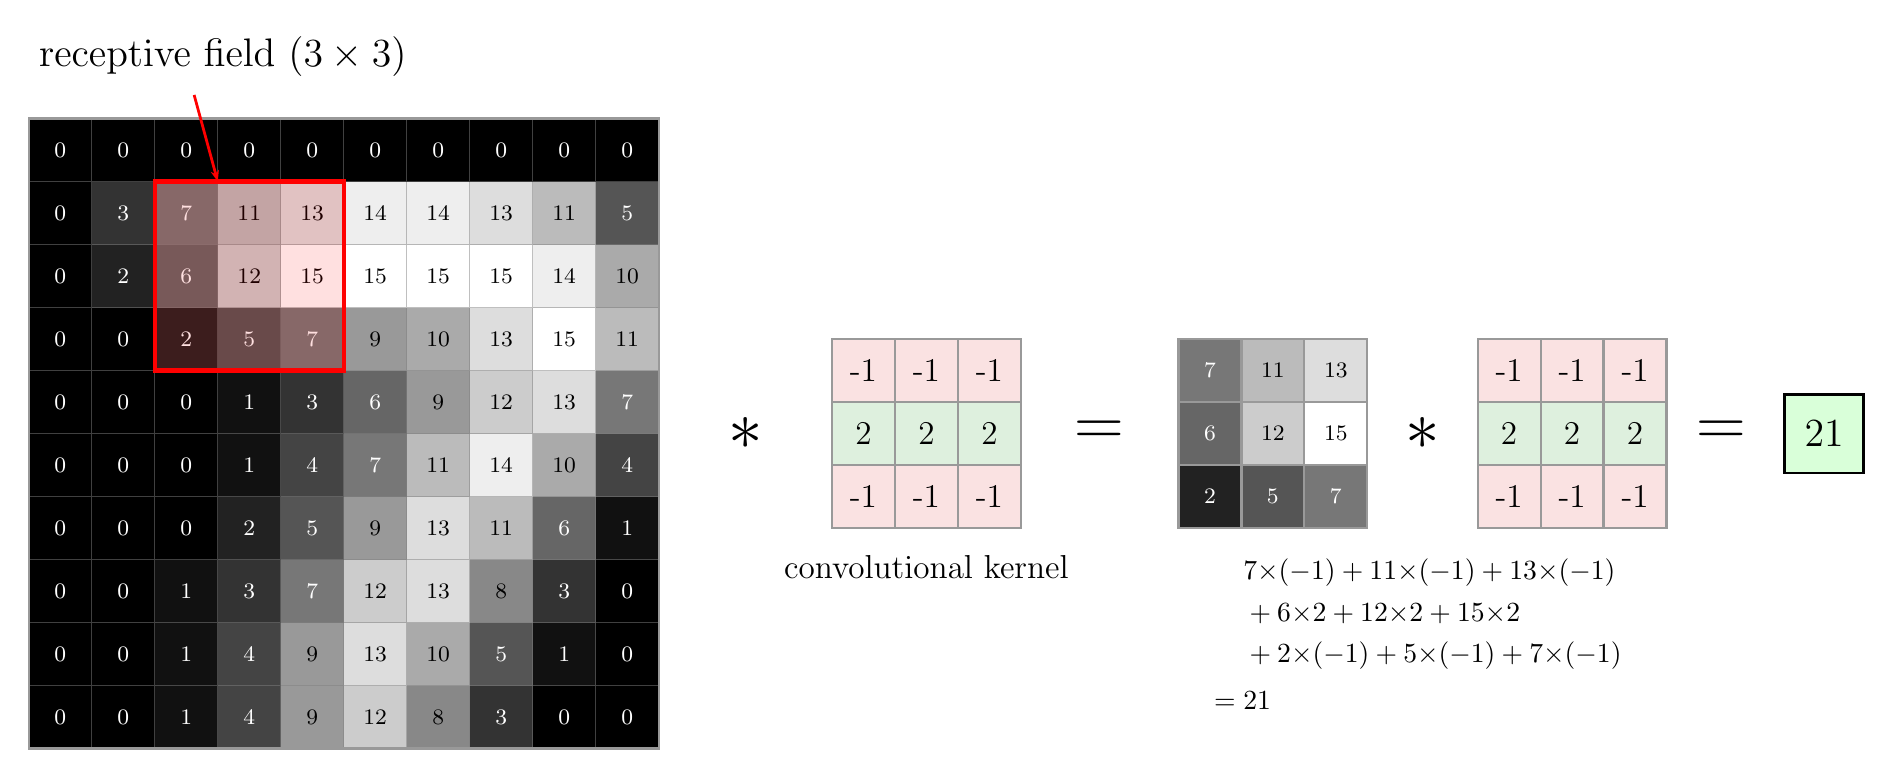
\begin{tikzpicture}[>={Stealth[length=4pt]}, line width=0.8pt, font=\large]

  % ========== 可复用：带数字的 10x10 图（#1 = 左下角 y 偏移） ==========
  \newcommand{\drawimage}[1]{%
    \foreach \v [count=\n] in {%
      0,0,0,0,0,0,0,0,0,0,%
      0,3,7,11,13,14,14,13,11,5,%
      0,2,6,12,15,15,15,15,14,10,%
      0,0,2,5,7,9,10,13,15,11,%
      0,0,0,1,3,6,9,12,13,7,%
      0,0,0,1,4,7,11,14,10,4,%
      0,0,0,2,5,9,13,11,6,1,%
      0,0,1,3,7,12,13,8,3,0,%
      0,0,1,4,9,13,10,5,1,0,%
      0,0,1,4,9,12,8,3,0,0%
    }{%
      \pgfmathtruncatemacro{\col}{int(mod(\n-1,10))}
      \pgfmathtruncatemacro{\row}{int((\n-1)/10)}
      \pgfmathsetmacro{\gpct}{\v/15}
      \definecolor{px}{gray}{\gpct}
      \fill[px] ({0.8*\col}, {#1+0.8*(9-\row)}) rectangle ++(0.8,0.8);
      \ifnum\v>7 \def\tc{black}\else \def\tc{white}\fi
      \node[font=\footnotesize, text=\tc] at ({0.8*\col+0.4}, {#1+0.8*(9-\row)+0.4}) {\v};
    }
    \begin{scope}[shift={(0,#1)}]
      \draw[gray, opacity=0.5, thin, step=0.8] (0,0) grid (8,8);
      \draw[gray!80] (0,0) rectangle (8,8);
    \end{scope}
    \fill[red, opacity=0.12] (1.6, {#1+4.8}) rectangle (4.0, {#1+7.2});
    \draw[red, line width=1.6pt] (1.6, {#1+4.8}) rectangle (4.0, {#1+7.2});
  }

  % ========== 可复用：卷积核 3x3 ==========
  \newcommand{\drawkernel}[2]{%
    \foreach \w [count=\m] in {-1,-1,-1,2,2,2,-1,-1,-1} {%
      \pgfmathtruncatemacro{\kc}{int(mod(\m-1,3))}
      \pgfmathtruncatemacro{\kr}{int((\m-1)/3)}
      \ifnum\w>0 \definecolor{kw}{RGB}{222,240,222}\else \definecolor{kw}{RGB}{250,226,226}\fi
      \fill[kw] ({#1+0.8*\kc}, {#2+1.6-0.8*\kr}) rectangle ++(0.8,0.8);
      \node[font=\large] at ({#1+0.8*\kc+0.4}, {#2+1.6-0.8*\kr+0.4}) {\w};
    }
    \begin{scope}[shift={(#1,#2)}]
      \draw[gray!80, step=0.8] (0,0) grid (2.4,2.4);
      \draw[gray!80] (0,0) rectangle (2.4,2.4);
    \end{scope}
  }

  % ========== 可复用：提取出的 3x3 图像块 ==========
  \newcommand{\drawwin}[2]{%
    \foreach \v [count=\m] in {7,11,13,6,12,15,2,5,7} {%
      \pgfmathtruncatemacro{\wc}{int(mod(\m-1,3))}
      \pgfmathtruncatemacro{\wr}{int((\m-1)/3)}
      \pgfmathsetmacro{\gpct}{\v/15}
      \definecolor{px}{gray}{\gpct}
      \fill[px] ({#1+0.8*\wc}, {#2+1.6-0.8*\wr}) rectangle ++(0.8,0.8);
      \ifnum\v>7 \def\tc{black}\else \def\tc{white}\fi
      \node[font=\footnotesize, text=\tc] at ({#1+0.8*\wc+0.4}, {#2+1.6-0.8*\wr+0.4}) {\v};
    }
    \begin{scope}[shift={(#1,#2)}]
      \draw[gray!80, step=0.8] (0,0) grid (2.4,2.4);
      \draw[gray!80] (0,0) rectangle (2.4,2.4);
    \end{scope}
  }

  % ================= 单行：图 x 核 = 3x3 x 3x3 = 结果 =================
  \drawimage{0}
  % 红框 -> receptive field 标注
  \node[font=\Large, anchor=south west] at (0,8.4) {receptive field ($3\times3$)};
  \draw[red, ->, line width=1pt] (2.1,8.3) -- (2.4,7.2);

  \node[font=\Huge] at (9.1,4) {$\ast$};
  \drawkernel{10.2}{2.8}
  % 卷积核标注
  \node[align=center] at (11.4,2.3) {convolutional kernel};

  \node[font=\Huge] at (13.6,4) {$=$};
  \drawwin{14.6}{2.8}
  \node[font=\Huge] at (17.7,4) {$\ast$};
  \drawkernel{18.4}{2.8}
  \node[font=\Huge] at (21.5,4) {$=$};
  \node[draw, line width=1pt, fill=green!15, minimum size=1cm, font=\Large]
    at (22.8,4) {21};

  % 具体计算过程：两个小矩阵下方，直接等号出结果
  \node[align=center, font=\normalsize] at (17.7,1.4) {%
    $\begin{aligned}
    & 7{\times}(-1)+11{\times}(-1)+13{\times}(-1) \\
    & +6{\times}2+12{\times}2+15{\times}2 \\
    & +2{\times}(-1)+5{\times}(-1)+7{\times}(-1) \\[2pt]
    ={} & 21
    \end{aligned}$
  };
\end{tikzpicture}
\end{document}